\section{Locking using ULI}\label{sec:lock}

In this section, we explain two different locking schemes using ULIs. In the
first scheme, each core executes its own critical section, while in the second
scheme, server cores are designated per lock to execute the critical section
protected by the lock on behalf of other cores.

\begin{figure}
\begin{code} 
void mylock(struct lock *L)
{
    int my_id  = GETMYID();
    int save_id;
    bool *my_trigger;
    struct args arg;
    message *msg = our_allocate();

    my_trigger = get_trigger(my_id);

    if (L->owner_id == -1)
retry:
        __sync_val_compare_and_swap(&L->owner_id, -1, my_id);

    __sync_synchronize();

    if ((L->owner_id != my_id)) {
        if (L->owner_id == -1) {
            goto retry;
        } else {
            arg.L = L;
            arg.ask_id = my_id;
            msg->callback = &addme;
            msg->param = arg;
            save_id = L->owner_id;
            if (save_id == -1)
                goto retry;
            SENDI(msg, save_id);
            while (!(*my_trigger));
        }
    }
    *my_trigger = 0;
}

void myunlock(struct lock *L)
{
    bool *next_trigger;
    int my_id = GETMYID();

    DUI(1);
    if (pcpu_lock_struct[my_id].waiter_id != -1) {
        next_trigger = get_trigger(pcpu_lock_struct[my_id].waiter_id);
        *next_trigger = 1;
        pcpu_lock_struct[my_id].waiter_id = -1;
    } else {
        L->owner_id = -1;
    }

    EUI(0xfffe);
}
\end{code}
\caption{Locking using ULI\label{fig-locking}}
\end{figure}

\subsection{Locking scheme 1}

Since interrupts are sent and received on cores, the core id is an important
parameter in this scheme. A lock structure is associated with an owner which is
the id of the core owning the lock currently. Every other core which requests
the lock will be put on an implicit queue of waiters in the order of their
requests. It is an implicit queue due to the following design.

When a core wants a lock, it sends an interrupt to the owner. The owner assigns
this core as its waiter. More importantly it hands over the ownership of the
lock to this waiter. It is important to note that, handing over ownership is not
equivalent to handing over control of the critical section. This happens only
when the old owner releases the lock and 'triggers' its waiter. When a second
core wants the lock it sends an interrupt to the new owner and the process is
repeated as above. One can therefore see that there is a queue of waiters being
formed with the ownership being passed on to the tail of the queue. This ensures
fairness of the locking scheme. Figure~\ref{fig-locking} displays the lock,
unlock primitives for this scheme. Each of the above steps is explained in
detail below with the help of this figure.

\subsubsection{Acquiring the lock}

The function mylock() is called by the cores wanting to enter the critical
section. Each core tries to set the ownership of the lock if it is not yet owned
by any other core and checks to see if it indeed got the lock. A barrier in
between these two steps ensures that every core sees a consistent value of the
lock owner at the end of the check. If a core wins the race to the ownership of
the lock it can continue into the critical section, else it has to convey to the
owner that it is waiting on the lock. It is important to note that the lock can
get released anytime during this entire process. In this case the core tries to
take the lock again.

\subsubsection{Sending ULI}

If a core fails to get a lock, it sends an interrupt to the owner of the lock
through the SENDI-Send Interrupt instruction, by passing a parameter containing
its id, pointer to the lock in question and the handler to be invoked by the
recipient of the interrupt. All of this is packaged into a message data
structure. One can see that our design allows every inter-processor ULI to be
associated with its own handler.  The core then spins on a per-cpu variable
which gets triggered when the lock is released. This ensures that every core
spins on its own cacheline thereby preventing cache contention which is a
primary source of performance degradation in many locking schemes.

\begin{figure}
\begin{code} 
static void addme(void *p)
{
    int my_id = GETMYID();
    struct args *arg = (struct args *)p;
    struct lock *L = (struct lock *)arg->L;
    int ask_id = (int)arg->ask_id;
    int save_id;
    message *msg = our_allocate();

    DUI(1);
retry:
    if (L->owner_id != my_id) {
        if (L->owner_id == -1) {
            __sync_val_compare_and_swap(&L->owner_id, -1, ask_id);

            __sync_synchronize();

            if (L->owner_id != ask_id) {
                msg->callback = &addme;
                msg->param = p;
                save_id = L->owner_id;
                if (save_id == -1)
                    goto retry;
                SENDI(msg, save_id);
            } else {
                bool *next_trigger = get_trigger(ask_id);
                *next_trigger = 1;
            }
        } else {
            msg->callback = &addme;
            msg->param = p;
            save_id = L->owner_id;
            if (save_id == -1)
                goto retry;
            SENDI(msg, save_id);
        }
    } else {
        L->owner_id = ask_id;
        pcpu_lock_struct[my_id].waiter_id = ask_id;
    }
    EUI(0xfffe);
}
\end{code}
\caption{Handling ULI\label{fig-locking_cont}}
\end{figure}

\subsubsection{Handling ULI}

The function addme() shown in Figure~\ref{fig-locking_cont} is the handler that
gets invoked on a SENDI. If the core that received the interrupt is indeed the
owner, it designates the sender of the interrupt as the lock owner, but does not
trigger the variable that the sender is waiting on. This is so that any further
requests for the lock is passed on to the next waiter in the queue to maintain
fairness. However, if the receiver of the interrupt is not the lock owner, it
sends an interrupt to the lock owner by forwarding it the same message that it
received. It is possible that the lock is released between the time that the
interrupt is sent and it is received. In this case, steps similar to the one in
mylock() is repeated, except, on the behalf of the waiter. Throughout the
handling, interrupts need to be disabled just as in normal interrupt handling
to avoid race conditions. This is done by the instructions DUI-Disable ULI,
EUI-Enable ULI

\subsubsection{Releasing the lock}

When the owner of the lock releases the lock in myunlock(), it checks to see if
it has pending waiters and sets the percpu parameter that the waiter is spinning
on. Otherwise it can reset the lock owner. Here too, since the lock->waiter\_id
and its percpu trigger are being manipulated, it is required to disable
interrupts throughout this function. We do not want the check on the waiter\_id
and the set on the trigger to happen on two different cores as a consequence of
receiving interrupts.

DUI, EUI and SENDI are the instructions that should be implemented by a system
with support for user level interrupts. Further ahead, we show how we emulate
these on baremetal. The section on simulation explains how such a system was
designed on Gem5.

\subsubsection{Emulating SENDI, DUI, EUI}

Each time an interrupt is sent, the message packet is queued on a percpu linked
list. When an interrupt is received, the core services each message packet from
this linked list. Disabling interrupts sets a percpu interrupt flag and EUI clears
the flag. We have designated a flag for ULIs with each bit intending to represent
a specific type of ULI.  In this case, we designate the lowermost bit as the
interprocessor ULI which gets set and cleared. These flags are essential for
emulating receiving of interrupts which is explained below..

\subsubsection{POLL}

We emulate delivery of interrupt by interleaving POLL in between the code. A
call to POLL checks if the interrupt flag described above is enabled and if so
dequeues the messages from the list created by SENDI and handles them.  It is at
this point that the handler embedded within the message is invoked as described
in Section 4.3.

\subsubsection{Limitations}

Every thread must have a 1-1 mapping with a core in the system. This is because
the scheme associates a lock owner, waiter and trigger parameters with a cpu id.
If a waiter thread is scheduled on another core, the trigger may be set on the
core that it previously ran on. If a lock owner thread is scheduled on another
core, all interrupts from waiters may go to a different core. This is the case
even when multiple threads are scheduled on the same core. We can overcome this
by transforming the design from a per-cpu to a per-process one. However, this is
not the focus of this paper.

\subsection{Locking scheme 2}

This scheme is inspired by the Remote Core Locking Mechanism a.k.a RCL lock
whose aim is to reduce lock contention by designating a server core to handle
critical sections on the behalf of other cores \cite{lozi}. This also helps improve locality
for the critical section since a dedicated core is in charge of executing
critical sections. 

\subsubsection{RCL lock overview}

The critical sections are converted into function calls so as to be executed on
the server core as remote procedure calls. Similar to a function, they are
associated with input parameters and return values. Every client core inserts
the address of the function to be executed, the input parameters in an array and
waits for the server core to reset the address of the function to NULL. The
array is aligned such that each entry falls into a percpu cacheline. The server
core iterates through the array, executes a function at a time and sets the
address of the function in the slot to NULL, which tells the client that the
server has executed the critical section.

This means that the server core is busy iterating through this array all the
time without being able to do any other useful work. ULIs can help avoid this
problem as is described below.

\subsubsection{Using ULIs to implement RCL locks}

Each time a client inserts a function to be executed on the server it can send a
ULI to the server core by passing a message containing its core id. The server
services the interrupt by executing the function in the slot equal to the core
id that was passed by the client. This ensures that the server can continue to
do useful work while it services the clients. We can in fact now dedicate one
lock per core and distribute the traffic because the server is capable of
handling work besides just servicing the remote critical sections. This design
can be used in any locking scheme that uses the client server model of locking.

\section{Lazy thread using ULI}

In this section, we are going to implement lazy thread \cite{goldstein} using ULI. We will first introduce the concept of lazy thread and stacklet. Then we will explain in detail how we use ULI to implement lazy thread in the case of two parallel sequential calls followed by a join.

\subsection{Lazy thread overview}
Lazy thread is a compilation technique to reduce the burden of programmers for multicore architectures. The problem this technique tries to solve is how to reduce the overhead of excessive parallelism when the hardware cannot consume. When the programmer has a multicore machine and a problem to solve, he needs to first exploit parallelism of the problem, then he needs to decide how many threads to create and in what fashion to dispatch the parallelism. This complexity also increases the maintenance cost of the software, as the software needs to be rewrite for best performance when the underlying hardware changes. With lazy thread, the programmer can create as many parallel calls as he wants without worrying the overhead of the parallel calls.

The way lazy thread works is that it turns parallel calls into normal function calls while preserve the ability of elevating a normal function call back to a parallel call. We call these special normal function calls \textbf{parallel sequential call}. That is, before a parallel sequential call gets called, if no other cores become idle and steal the work, then the parallel sequential call will become a normal function call. Otherwise the idle core will steal the work by creating a \textbf{stacklet} and execute the work.

A stacklet is a piece of dynamic allocated area used as a stack. The difference between a stacklet and a normal stack is the first function in a normal stack will never return, whereas the first of a stacket will return and the program counter and stack pointer will be changed to the parent of this stacklet. Stacklet makes it possible to elevate a parallel sequential call, which is represented by a seed, into a real parallel call.

As the overhead of a parallel sequential call, if being executed as a normal function call, is almost zero, and the overhead of elevating a parallel sequential call to a real parallel call is no more than traditional parallel call, lazy thread allows programmers to program in multicore environment with ease and makes software compatible even the hardware changes.

Now, with the help of ULI, you will notice in the following implementation of lazy thread we do not have a single shared lock between cores. As we add more cores to computation, the lock contention problem will not occur. This gives us a extensible parallel computing framework.

\subsection{Implementation of lazy thread}
We will show how to implement lazy thread when we have two parallel calls followed by a join. Assume we have a naive fibonacci function recursively calculates its value.
\begin{figure}
\begin{code}
int fib(int n) {
    if (n <= 2) return n;
    int a = parallel call fib(n-1);
    int b = parallel call fib(n-2);
    return a + b;
}
\end{code}
\caption{Naive fibonacci function}
\end{figure}

This function will for sure performs badly because it is creating too many threads and the overhead of thread creation is a lot greater than the work itself. Now we can compile this code, using lazy thread compilation technique, into much more efficient code as the figure shows in a high level representation. ss* in this figure means seed stack.

Now we are going to describe what would happen for each SENDI in the graph.

\begin{figure}
\centering
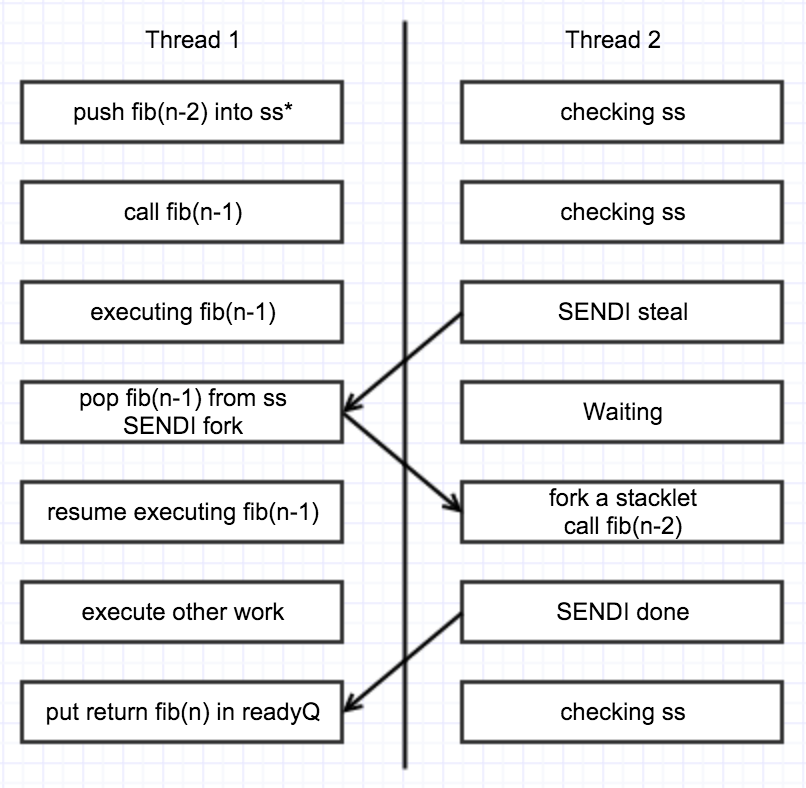
\includegraphics[width=0.6\textwidth]{../hongliy/stacklet}
\caption{Lazy thread with ULI}
\end{figure}

\subsubsection{SENDI steal}
At beginning, thread 1 starts executing fib(n), while thread 2 has no work to do thus it consistently checks the \textbf{seed stack}. A seed stack is a per-thread struct that stores the information (or \textbf{seed}) of the parent function frame's stack pointer and the pc of a code segment which does a piece of work, for example, here the work is to steal the seed. Thread 1 will first push the work of fib(n-2), which is the second parallel sequential call, into the seed stack. Then thread 1 will calls fib(n-1) just like a normal function call. While thread 1 is executing fib(n-1), thread 2 notice there is some work in thread 1's seed stack, so it will use SENDI to send a message to ask thread 1 to give the work to thread 2.

\subsubsection{SENDI fork}
After thread 1 receives the message from thread 2, it is going to the interrupt handler for steal. It will first pop the seed from the seed stack. It will also change the return address of fib(n-1) so thread 1 will skip executing fib(n-2). Then thread 1 will send a message to thread 2 to ask it to fork a stacklet and execute fib(n-2). After this, thread 1 resumes its work and thread 2 will start to execute fib(n-2).

\subsubsection{SENDI done}
After thread 2 finishes executing fib(n-2), it will send a message telling thread 1 the work is done. Let's assume thread 1 has already finished fib(n-1) and is currently doing something else. So thread 1 will go into interrupt handler for done. In the handler, thread 1 will put the the fact that fib(n) has been completed (fib(n-1) has been executed in thread 1 and fib(n-2) has been executed in thread 2) into a \textbf{ready queue}. Thread 1 will later check the ready queue to resume any work in there.

